\documentclass[12pt,a4paper]{article}
\usepackage[margin=2cm]{geometry}
\usepackage{graphicx}
\usepackage{enumitem}
\usepackage{hyperref}
\usepackage{fancyhdr}
\usepackage{titlesec}
\usepackage{xcolor}
\usepackage{float}
\usepackage{amsmath}
\setlength{\headheight}{15pt}

\pagestyle{fancy}
\fancyhf{}
\rhead{Drone Mapper -- High Level Design}
\lhead{Advanced Topics in Programming 2026B}
\cfoot{\thepage}

\titleformat{\section}{\Large\bfseries}{}{0em}{}
\titleformat{\subsection}{\large\bfseries}{}{0em}{}
\titlespacing*{\section}{0pt}{8pt}{4pt}
\titlespacing*{\subsection}{0pt}{6pt}{3pt}

\begin{document}

\begin{center}
{\LARGE\bfseries High Level Design Document}\\[4pt]
{\Large Drone Mapper -- Exercise 1}\\[8pt]
{\large Advanced Topics in Programming, Semester B 2026}\\[12pt]
\begin{tabular}{ll}
\textbf{Name} & \textbf{ID} \\
\hline
Almog Tavor & (ID: 323084962) \\
Yonatan Kahana & (ID: 212223036) \\
\end{tabular}
\end{center}

\vspace{6pt}

\section{1. UML Class Diagram}

The diagram below shows the main classes, their relationships, and key
methods. Interfaces are blue, core classes yellow, mock implementations
green, data types pink, and utilities purple.

\vspace{2pt}
\begin{center}
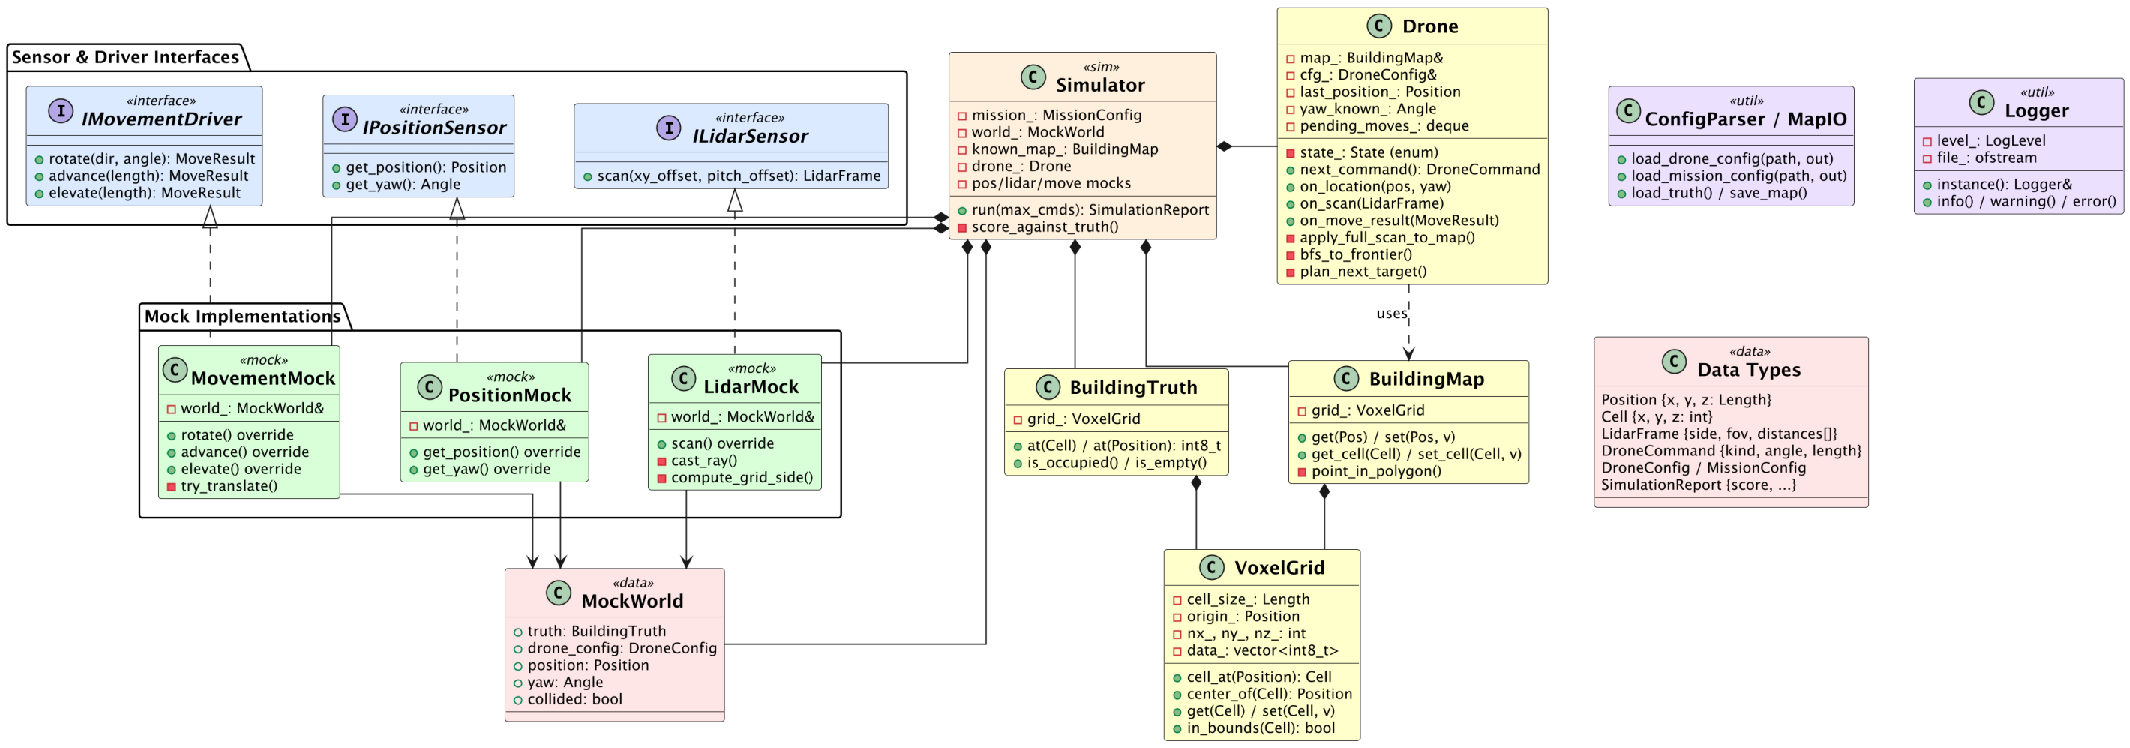
\includegraphics[width=\textwidth,height=0.7\textheight,keepaspectratio]{class_diagram.pdf}
\end{center}

\vspace{-4pt}
\noindent Key relationships:
\begin{itemize}[nosep,topsep=2pt]
\item \textbf{Simulator} owns all mocks, the Drone, both maps, and orchestrates the loop.
\item \textbf{Drone} sees only abstract interfaces (ILidarSensor, IPositionSensor,
      IMovementDriver) through the command/response pattern -- it never touches the
      mocks or truth directly.
\item \textbf{MockWorld} is shared state between the three mocks so that movement
      updates are visible to the position and lidar sensors.
\item \textbf{VoxelGrid} is the shared spatial data structure, composed into both
      BuildingTruth and BuildingMap.
\end{itemize}

\newpage
\section{2. UML Sequence Diagram -- Main Flow}

The diagram shows the four phases of the main simulation loop: location
query, scanning, movement, and scoring.

\vspace{2pt}
\begin{center}
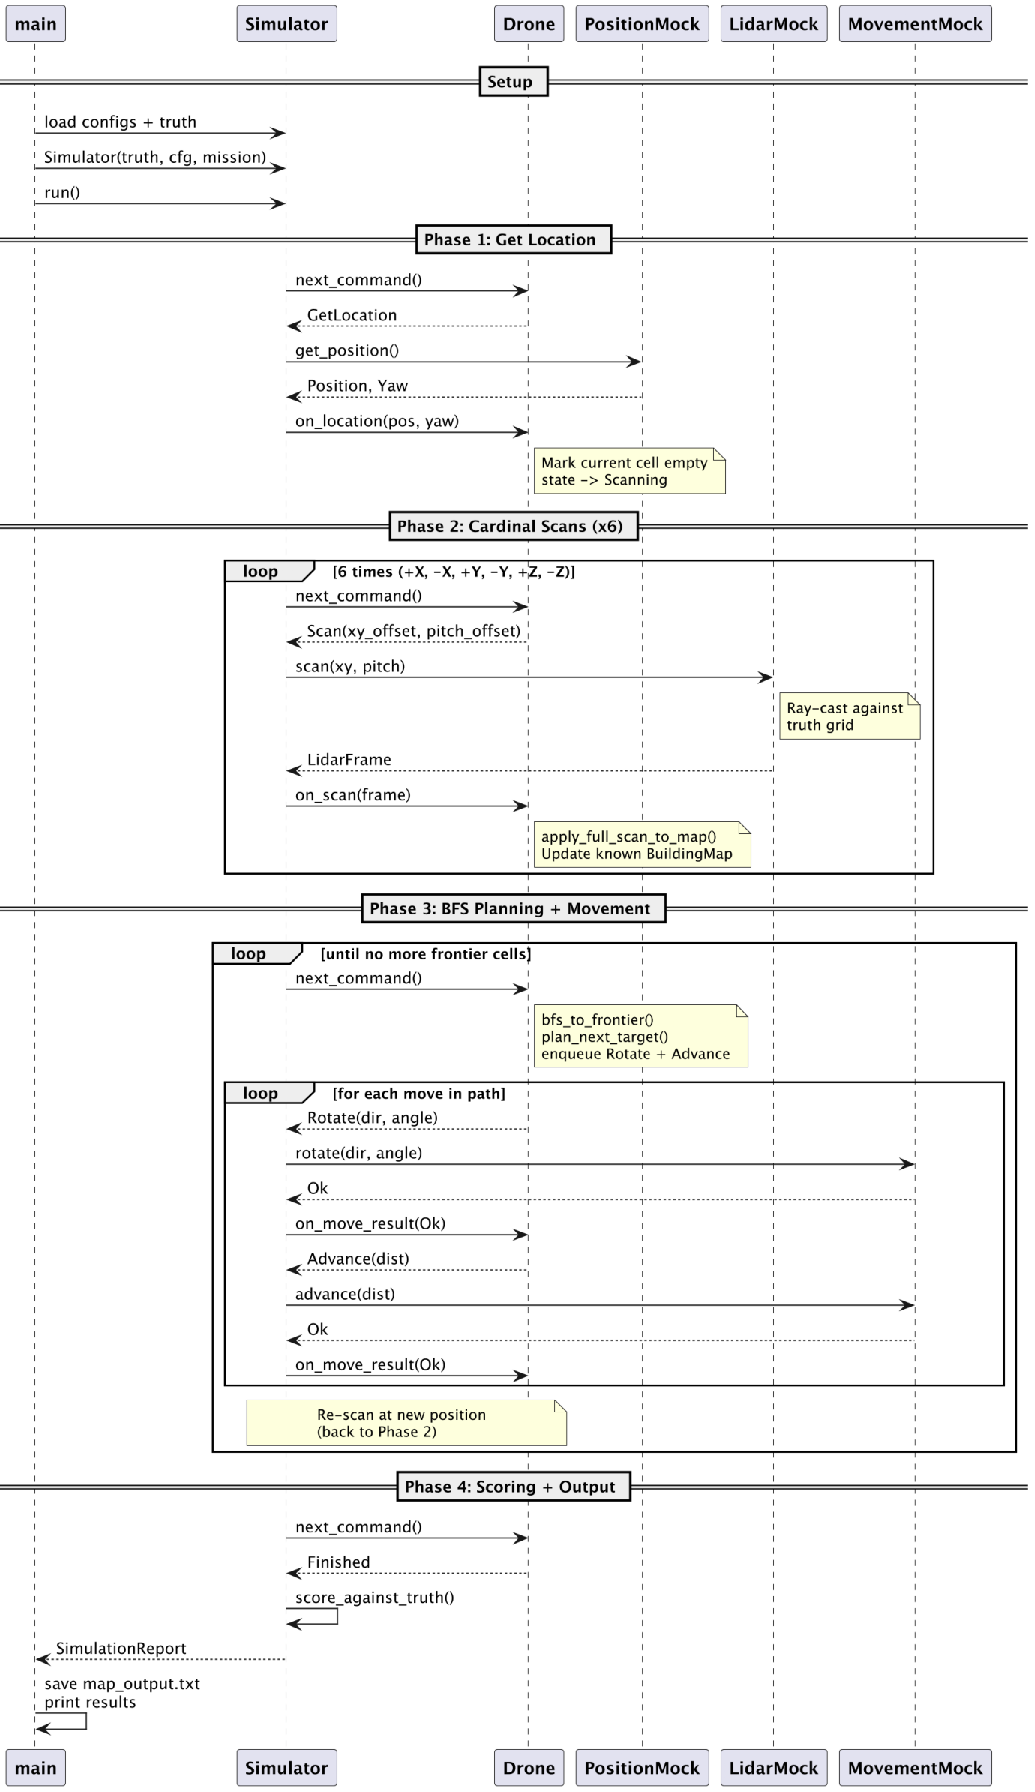
\includegraphics[width=\textwidth,height=0.85\textheight,keepaspectratio]{sequence_diagram.pdf}
\end{center}

\newpage
\section{3. Design Considerations and Alternatives}

\subsection{3.1 Separation of Drone Logic from Simulation}

The drone never directly accesses the building truth or the mock implementations.
Instead, the \textbf{Simulator} acts as a mediator: it asks the Drone for a
command, dispatches it to the appropriate mock, and feeds the result back. This
mirrors a real embedded system where the flight controller issues commands and
receives sensor data through hardware abstraction layers.

\textbf{Alternative considered:} Letting the drone call sensor/driver interfaces
directly (dependency injection). We rejected this because the assignment's ``main
loop'' specification explicitly requires the simulator to ask the drone for
commands, making the command-response pattern the natural fit.

\subsection{3.2 Voxel Grid as Shared Spatial Representation}

Both \texttt{BuildingTruth} and \texttt{BuildingMap} wrap the same
\texttt{VoxelGrid} class. This ensures identical coordinate-to-cell mapping
and makes the scoring comparison straightforward (iterate both grids in lock-step).

\textbf{Alternative considered:} Using an octree or sparse hash map for the
drone's known map (since most cells start as ``unmapped''). We chose a dense
grid for simplicity and because the building sizes in exercise~1 are small
enough that memory is not a concern.

\subsection{3.3 Lidar Beam Geometry (Circles of Beams)}

The lidar follows the assignment specification's beam geometry:
\begin{itemize}[nosep]
\item \textbf{Circle 0} is a single central beam fired along the scan centerline.
\item \textbf{Circles 1..FOVC-1} are concentric rings of $4^k$ evenly-spaced
      beams. Ring $k$ has radius $k\cdot D$ at distance Z-min, so its cone
      half-angle is $\arctan(k\cdot D / \text{Z-min})$.
\item Each beam reports: distance to the closest hit if $\ge$ Z-min,
      \texttt{0} if the hit is closer than Z-min (per spec), and \texttt{-1}
      if no hit occurred within Z-max (kept so the mock can return one
      record per emitted beam as allowed by the Ex1 clarification).
\end{itemize}

After every scan the drone back-projects each beam's direction (azimuth +
elevation relative to the centerline) into world space, walks the voxel
cells along the ray, marks intermediate cells \texttt{kEmpty}, and marks
the hit cell \texttt{kOccupied} when the beam terminates on an obstacle.

\textbf{Alternative considered:} An axis-aligned ray matrix (one ray per
$(\text{row}, \text{col})$ in a square grid covering the FOV). It was simpler
to implement but diverges from the spec's explicit ring geometry; we replaced
it once the spec required FOVC/D-driven beam counts.

\subsection{3.4 Frontier-Based BFS Exploration}

The drone maintains a ``frontier'' -- known-empty cells adjacent to unmapped
cells. At each waypoint it runs BFS through known-empty cells to find the
nearest frontier, plans the shortest path, and follows it. This is complete
(it will visit every reachable cell) and deterministic (BFS neighbor order
is fixed).

\textbf{Alternative considered:} DFS / wall-following. DFS is simpler but can
lead to long back-tracking paths. A\textsuperscript{*} with distance heuristic
could reduce path lengths but adds complexity without material benefit at
exercise~1 grid sizes.

\subsection{3.5 Strong Types with mp-units}

All values and APIs use the mp-units library (v2.0.0) as required by the
assignment. A thin wrapper header (\texttt{include/units/Units.h}) includes
mp-units and provides \texttt{Length} and \texttt{Angle} type aliases plus
\texttt{using} declarations for \texttt{cm}, \texttt{m}, and \texttt{deg}.
This keeps downstream code concise (\texttt{5.0 * cm}, \texttt{90.0 * deg})
while mp-units enforces dimensional safety at compile time.

mp-units is resolved through the course's vcpkg toolchain
(\texttt{vcpkg.json} declares the dependency; the CMake build calls
\texttt{find\_package(mp-units CONFIG REQUIRED)}). This matches the
build setup used by the teacher's reference \texttt{example\_mock\_lidar}
project. gsl-lite is pulled in transitively by mp-units.

\subsection{3.6 Rectangle Boundary and Single-Resolution Policy}

Per the assignment spec, the mission boundary is a bounded rectangle
(\texttt{min\_x}, \texttt{max\_x}, \texttt{min\_y}, \texttt{max\_y}) combined
with a vertical range (\texttt{height\_min}, \texttt{height\_max}). The
\texttt{BuildingMap} constructor pre-marks every cell whose center falls
outside this volume as \texttt{kOutOfBounds} (-2), so the scoring stage and
the drone's exploration both naturally ignore those cells.

The mission also declares the requested mapping resolution
(\texttt{xy\_resolution\_cm}, \texttt{height\_resolution\_cm}). Per the Ex1
resolution clarification, we support a single resolution: the one used by
the input map (its \texttt{cell\_size}). If the requested resolution does
not match, the program prints a clear error and exits via \texttt{main}
without running the simulation.

\textbf{Note on drone shape:} The assignment's Ex1 clarification states the
drone may be modeled as a perfect sphere, which means rotation is
collision-free without environment checks. Our movement mock relies on
this: rotations only update yaw and never test the surrounding voxels.

\subsection{3.7 Floating-Point Position Snapping}

We discovered that cumulative floating-point drift from \texttt{cos($\pi$/2)}
not being exactly zero caused the drone's actual position to cross cell
boundaries, leading to incorrect lidar readings and infinite loops. The fix:
snap world position to the nearest 0.01\,cm after every movement in the mock.

\subsection{3.8 Error Recovery Strategy}

All input file errors are recoverable where possible: missing config keys use
defaults, malformed map rows are padded, and unknown keys are logged. Only truly
fatal errors (file not found, no grid data) cause the program to print an error
and exit via \texttt{main} return -- never via \texttt{exit()} or exceptions
escaping \texttt{main}.

\section{4. Testing Approach}

\subsection{4.1 Framework}

We use a custom dependency-free micro test framework (\texttt{tests/test\_framework.h})
that provides \texttt{TEST()}, \texttt{CHECK()}, \texttt{CHECK\_EQ()}, and
\texttt{CHECK\_NEAR()} macros. Tests are auto-registered and run sequentially
from a single \texttt{main()}.

\subsection{4.2 Test Layers}

\begin{center}
\small
\begin{tabular}{llp{7.5cm}}
\textbf{Layer} & \textbf{File (count)} & \textbf{What is tested} \\
\hline
Unit types & test\_units.cpp (4) & Length/Angle construction, arithmetic, normalization, radian conversion \\
Spatial data & test\_voxel\_grid.cpp (4) & Set/get, out-of-bounds, continuous-to-cell conversion, origin offset \\
Known map & test\_building\_map.cpp (2) & Rectangle boundary marking, height-range filtering \\
Config I/O & test\_config\_parser.cpp (4) & Drone capabilities parse, unknown key recovery, mission rectangle, missing file \\
Map I/O & test\_map\_io.cpp (3) & Load truth, round-trip save/load, missing file \\
Lidar mock & test\_lidar\_mock.cpp (3) & Central beam hits end wall, total beam count matches $1+\sum 4^k$, open-direction returns $-1$ \\
Movement mock & test\_movement\_mock.cpp (4) & Advance direction, rotate yaw, wall collision, max clamping \\
Drone logic & test\_drone.cpp (2) & Initial GetLocation command, scan sequence after location \\
Integration & test\_simulator.cpp (2) & Full simulation of small room ($\ge$80\% score); sealed pocket (no collision) \\
\hline
& \textbf{Total: 28 tests} &
\end{tabular}
\end{center}

\subsection{4.3 Testing Strategy}

\begin{itemize}[nosep]
\item \textbf{Bottom-up:} Each module is tested in isolation before integration.
      Mocks are tested against known truth grids with predictable geometry.
\item \textbf{Integration:} The two simulator tests create a full
      truth$\to$simulator$\to$drone pipeline and verify end-to-end behaviour
      (score threshold, no collisions).
\item \textbf{Error paths:} Config parser tests verify that missing files,
      unknown keys, and malformed values are handled gracefully with recoverable
      defaults.
\item \textbf{Determinism:} All tests are deterministic (no randomness in the
      algorithm). Running the same input always produces the same output.
\item \textbf{Run:} \texttt{make test} builds and executes the entire suite.
\end{itemize}

\subsection{4.4 Sample Input Sets}

Three input sets exercise different scenarios:

\begin{enumerate}[nosep]
\item \textbf{set1} -- Simple 10$\times$10 empty room (baseline correctness).
\item \textbf{set2} -- 15$\times$12 building with a sealed 3$\times$3 pocket
      (tests that inaccessible areas remain unmapped without crashing).
\item \textbf{set3} -- L-shaped truth map within a $150\times150$ rectangle
      (tests that the rectangle boundary plus the spec's resolution policy
      correctly leave the non-L portion as unmapped, since the drone cannot
      reach it).
\end{enumerate}

\end{document}
